\documentclass[11pt]{beamer}
\usetheme{Warsaw}
\usepackage[utf8]{inputenc}
\usepackage{amsmath}
\usepackage{amsfonts}
\usepackage{amssymb}
\setbeamertemplate{footline}[frame number]%添加页码

\usepackage{fontspec}
\setsansfont{Charis SIL}%setmainfont对beamer没有用
%也可以使用以下命令
%\setmainfont(Charis SIL)
%\setfonttheme{serif}

\usepackage{booktabs}
\usepackage{polyglossia}
\setmainlanguage{french}
\usepackage{ctex}
\usepackage{makecell}
\usepackage{multirow}
\usepackage{xspace}
\usepackage{graphicx}
\usepackage{subcaption}
\usepackage{longtable} 
\usepackage{colortbl}
\usepackage{xcolor}
%\usepackage[colorlinks=true, linkcolor=blue, anchorcolor=blue, citecolor=blue]{hyperref}%beamer模式下不能使用这一个包

\usepackage[style=langsci-unified]{biblatex}
\addbibresource{SoutenanceRef.bib}
\DefineBibliographyExtras{french}{\renewcommand*\mkbibnamefamily[1]{#1}}
\DeclareFieldFormat*{titlecase}{#1}
\DeclareNameAlias{default}{family-given}
\renewcommand*{\multinamedelim}{\addspace\&\addspace}
\DefineBibliographyStrings{french}{editors = {éds\adddot}}
\DeclareFieldFormat{type}{\mkbibparens{\bibstring{#1}}}

\title{Constitution d'une base de données lexicales des langues sinitiques et contribution à l'étude de leur phylogénie}
\author{YIN Yuanhao (22100358)}
\institute{INALCO, SDL (M2) 

Parcours : Linguistique : langues, terrains, variations, typologie
}

\date{}
\logo{
\includegraphics[scale=.5]{inalco-logo-color}} 
%\setbeamercovered{transparent} 
%\setbeamertemplate{navigation symbols}{} 
%\subject{Soutenance}

\begin{document}

\begin{frame}
\titlepage
\end{frame}

\begin{frame}
\tableofcontents
\end{frame}

\section{Introduction}
\begin{frame}{La classification des langues sinitiques}
Les critères traditionnels : 
\begin{itemize}
\item{Les initiales obstruantes sonores du chinois moyen}

\item{Les syllabes à codas *-p/t/k du chinois moyen}
\end{itemize}

Questions :
\begin{itemize}
\item{Phonétique/phonologique}

\item{Rétention commune}

\item{Absence de la stratification}
\end{itemize}
\end{frame}


\begin{frame}{Exemple 1}
\textcite{li1987atlas} et \textcite{xiong2012atlas} : 
\begin{enumerate}
\item{Mandarin 官话}
\item{\textbf{Jin 晋语 (séparé du mandarin)}}
\item{Wu 吴语}
\item{Min 闽语}
\item{Hakka 客家话}
\item{Yue 粤语}
\item{Xiang 湘语}
\item{Gan 赣语}
\item{Hui 徽语}
\item{Pinghua et Patois 平话和土话}
\end{enumerate}
\end{frame}

\begin{frame}{Exemple 1}
Mandarin :
\begin{enumerate}
\item{Nord-est 东北}
\item{Beijing 北京}
\item{Jilu 冀鲁}
\item{Jiaoliao 胶辽}
\item{Zhongyuan 中原}
\item{Lanyin 兰银}
\item{Jianghuai 江淮}
\item{Sud-ouest 西南}
\end{enumerate}
\end{frame}

\begin{frame}{Exemple 1}
\textcite[A2]{li1987atlas} et \textcite[5]{Shen1994Taiyuan} : 

\resizebox{\textwidth}{!}{
    \begin{tabular}{lccccccc|c}
    \toprule
    \makecell{Initiales \\du MC} & \multicolumn{1}{l}{西南} & \multicolumn{1}{l}{中原} & \multicolumn{1}{l}{冀鲁} & \multicolumn{1}{l}{兰银} & \multicolumn{1}{l}{北京/东北} & \multicolumn{1}{l}{胶辽} & \multicolumn{1}{l|}{江淮} & \multicolumn{1}{l}{\makecell{Jin \\(Taiyuan)}} \\
    \midrule
    Sourde & 2     & 1     & 1     & 4     & 1234  & 3     & \cellcolor[rgb]{ .851,  .851,  .851}D & \cellcolor[rgb]{ .851,  .851,  .851}D1 \\
    Sonante & 2     & 1     & 4     & 4     & 4     & 4     & \cellcolor[rgb]{ .851,  .851,  .851}D & \cellcolor[rgb]{ .851,  .851,  .851}D2 \\
    Sonore & 2     & 2     & 2     & 2     & 2     & 2     & \cellcolor[rgb]{ .851,  .851,  .851}D & \cellcolor[rgb]{ .851,  .851,  .851}D2 \\
    \bottomrule
    \end{tabular}}%

Les tonèmes des syllabes à codas *-p/t/k du chinois moyen dans les variantes du mandarin
\end{frame}

\begin{frame}{Exemple 2}
\textcite{li2012pinghua} : 
\begin{enumerate}
\item{Mandarin 官话}
\item{Wu 吴方言}
\item{Xiang 湘方言}
\item{Min 闽方言}
\item{Yue 粤方言}
\item{Gan 赣方言}
\item{\textbf{Hakka 客家方言 (distinct du Gan pour des raisons culturelles)}}
\item{Pinghua平话}
\item{\textbf{Hui 徽州话 (de nature mélangée et transitionnelle)}}
\end{enumerate}
\end{frame}

\begin{frame}{Exemple 2}
\begin{scriptsize}
\textcite[511]{li2012pinghua} :
    \begin{tabular}{l|c|c|c|c}
    \toprule
    Tonème du MC & A     & B     & C     & D \\
    \midrule
    Mandarin & [pʰ]  & \multicolumn{3}{c}{[p]} \\
    Yue   & [pʰ]  & [pʰ]/[p] & \multicolumn{2}{c}{[p]} \\
    Xiang & \multicolumn{3}{c|}{[b] (majorité)/[p]} & [pʰ] (majorité)/[b] \\
    Wu    & \multicolumn{4}{c}{[b]} \\
    Hui (Jixi) & \multicolumn{4}{c}{[pʰ] (majorité)/[p]} \\
    Gan   & \multicolumn{4}{c}{[pʰ]} \\
    Hakka & \multicolumn{4}{c}{[pʰ]} \\
    Pinghua & \multicolumn{4}{c}{[p]} \\
    Min   & \multicolumn{4}{c}{[p] (majorité)/[pʰ]} \\
    \bottomrule
    \end{tabular}%
    
Les initiale obstruantes sonores du MC dans les langues sinitiques (prenons l'initiale [*b-] comme exemple) sans la stratification
\end{scriptsize}
\end{frame}

\begin{frame}{Exemple 2}
\begin{scriptsize}
    \begin{tabular}{l|c|c|c|c}
    \toprule
    Tonème du MC & A     & B     & C     & D \\
    \midrule
    Mandarin & [pʰ]  & \multicolumn{3}{c}{[p]} \\
    Taiyuan & \multicolumn{4}{c}{\cellcolor[rgb]{ .851,  .851,  .851}[p]} \\
    Rongcheng & \multicolumn{4}{c}{\cellcolor[rgb]{ .851,  .851,  .851}[p]} \\
    Yue   & \multicolumn{2}{c|}{[pʰ]} & \multicolumn{2}{c}{[p]} \\
    Xiang & \multicolumn{3}{c|}{[b]} & [pʰ] \\
    Wu    & \multicolumn{4}{c}{[b]} \\
    Hui (Jixi) & \multicolumn{4}{c}{[pʰ]} \\
    Gan   & \multicolumn{4}{c}{[pʰ]} \\
    Hakka & \multicolumn{4}{c}{[pʰ]} \\
    Pinghua & \multicolumn{4}{c}{[p]} \\
    Min   & \multicolumn{4}{c}{[p]} \\
    \bottomrule
    \end{tabular}%

Les initiale obstruantes sonores du MC dans les langues sinitiques (prenons l'initiale [*b-] comme exemple) pour les couches héritées
\end{scriptsize}
\end{frame}

\begin{frame}{La classification des langues sinitiques}
Les critères pour la phylogénie linguistique, une classification tant synchronique que diachronique :
\begin{itemize}
\item{Lexical}

\item{Innovation commune}

\item{Stratification}
\end{itemize}
\end{frame}

\begin{frame}
\textcite{sagart2011classifying} :
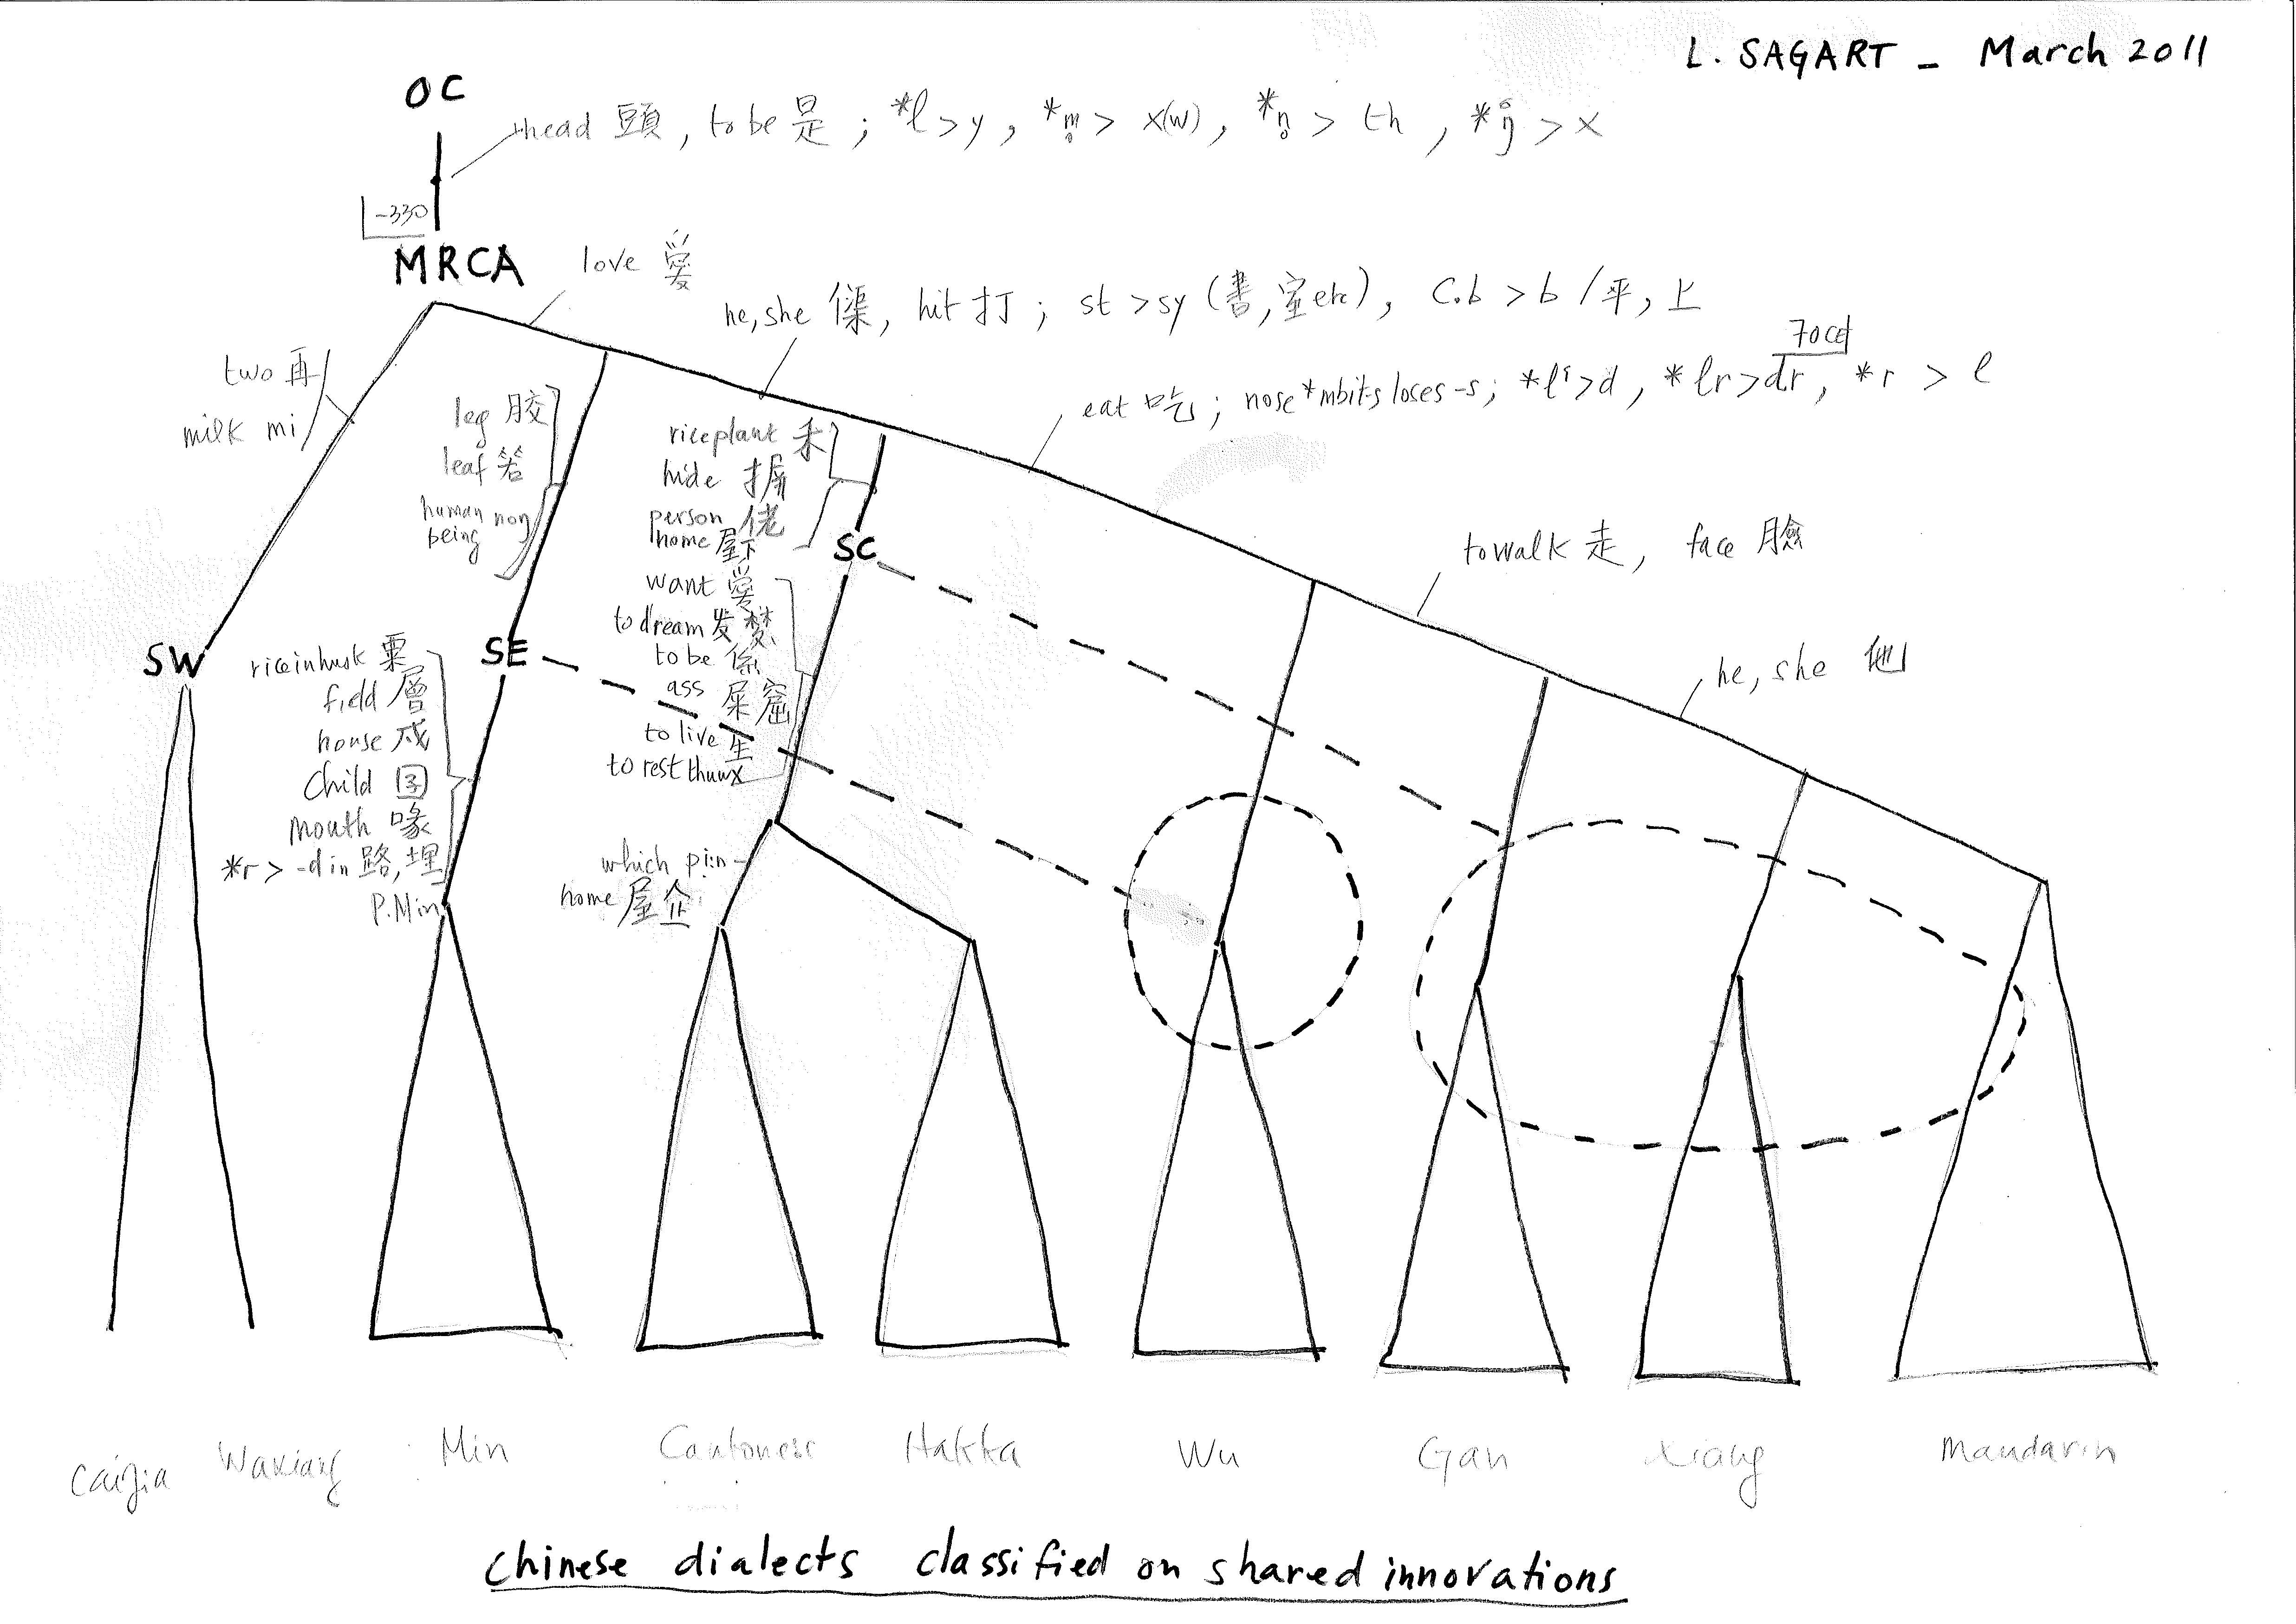
\includegraphics[scale=.25]{sagart}
\end{frame}

\section{Stratification}
\begin{frame}{Critères phonétiques de la stratification}
\textcite{Sagart2001hani}, \textcite{Chen2003yu} et \textcite{Chen2005couche} :
\begin{itemize}
\item{Correpondances phonétiques systématiques entre les doublets/triplets/quartets... sur une syllabe dans différents mots (``wen-bai'')}

\item{Connaissances de l'évolution phonologique du chinois (OC, MC, etc.)}

\item{Critère (étendu) de cohérence}
\end{itemize} 
\end{frame}
 
\begin{frame}{Exemple}
``日'' du Wu de Wenzhou :
\begin{itemize}
\item{couche I : [ne], ``三四\textasciitilde'' (\cite[158]{You1998Wenzhou}), ``trois ou quatre jours''}

\item{couche II : [ɲiai], ``生\textasciitilde'' (\cite[1471]{You1998Wenzhou}), ``anniversaire'' (couche héritée)}

\item{couche III : [zai], ``\textasciitilde 记'' (\cite[54]{Pan1998wenzhou}), ``journal intime''}
\end{itemize}
\end{frame}

\begin{frame}{Situations exceptionnelles}
\begin{itemize}
\item{\textcite{Cao2022tangxi} :

Les \textbf{mots grammaticaux} peuvent subir le changement phonétique exceptionnel (``fossilisation'', ``lénition'', etc.).

\begin{small}
e.g. ``去'' (``aller'', verbe directionnel), ``渠'' (prénom 3SG''), ``家'' (suffixe), etc.
\end{small}
}

\item{\textcite{Li1985diming} :

Les \textbf{toponymes} peuvent garder les prononciations archaïques.

\begin{small}
e.g. ``富''[pʰu] de ``大富车'' de la province du Hebei (\cite[36--37]{Wang2017diming_yixian})
\end{small}
}
\end{itemize}
\end{frame}

\section{Données}
\begin{frame}
Une base de données déjà établie par \textcite{wu2023annotating}

Traitement des données :
\begin{small}
\begin{itemize}
\item{Filtration des morphèmes non saillants, e.g. les suffixe ``子'', ``头'', etc.}

\item{Annotation des couches : 1 v.s. 2/3 pour Min et 2 v.s. 1/3/4 pour non Min}

\item{Correction de l'étymologie, e.g. ``拨'' > ``畀'' (``donner'') du Wu de Suzhou}

\item{Concepts à exclure (mal traduit, trop de variation, étymologie non déterminée, etc.)}

\item{COGIDs partielles (des syllabes) > COGIDs pleines (des mots)}
\end{itemize}
\end{small}
\end{frame}

\section{Phylogénie}
\begin{frame}{Méthodes phylogénétiques}
\textcite[74--75]{hall2018phylogenetic} et \textcite[15--16]{pellardfamily} :

\resizebox{\textwidth}{!}{
    \begin{tabular}{lllr}
    \toprule
          &       & Avantage & \multicolumn{1}{l}{Inconvénient} \\
    \midrule
    \multirow{3}[2]{*}{\makecell{Méthodes \\de diastances}} & UPGMA & rapide & \multicolumn{1}{l}{présupposition non pertinente} \\
          & NJ    &       &  \\
          & NN    &       &  \\
    \midrule
    \multirow{3}[2]{*}{\makecell{Méthodes \\de caractères}} & MP    & ``rule of thumb'' & \multicolumn{1}{l}{``long branch attraction''} \\
          & ML    &       & \multicolumn{1}{l}{chronophage} \\
          & BI    & populaire &  \\
    \bottomrule
    \end{tabular}}%

\hspace*{\fill}

On applique les méthodes d'UPGMA, d'NJ et de MP aux données suivant le tutoriel de M. Pellard\footnote{\url{https://tpellard.github.io/phylolinguistique/}}.
\end{frame}

\begin{frame}{UPGMA}
\begin{figure}[htbp]
\flushleft
\begin{subfigure}{.4\textwidth}
\centering
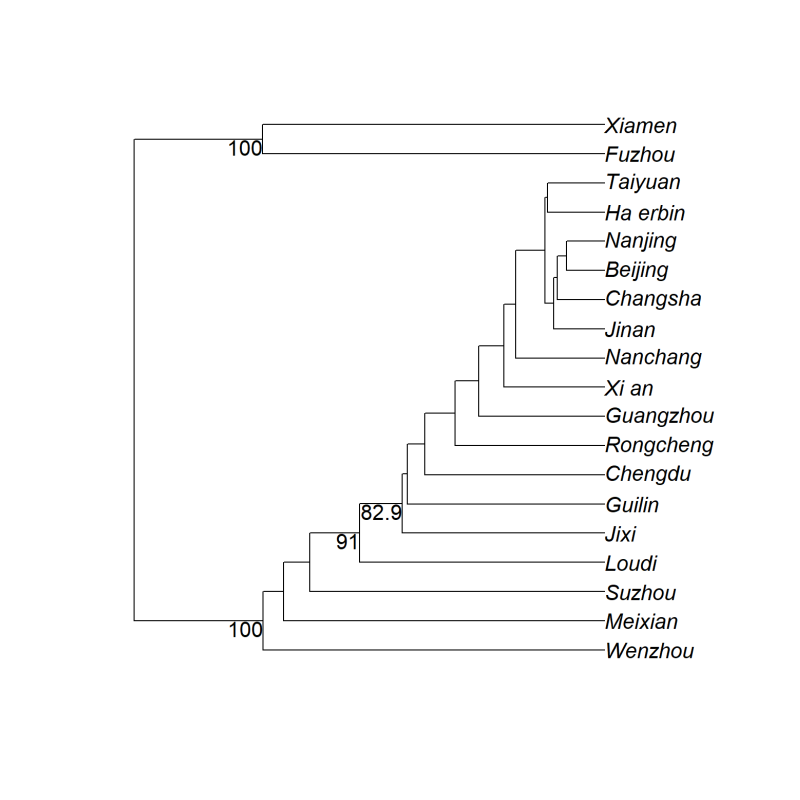
\includegraphics[scale=.2]{Figure/UPGMA_BS_with}
\caption{Avec emprunts}
\end{subfigure}
\begin{subfigure}{.4\textwidth}
\centering
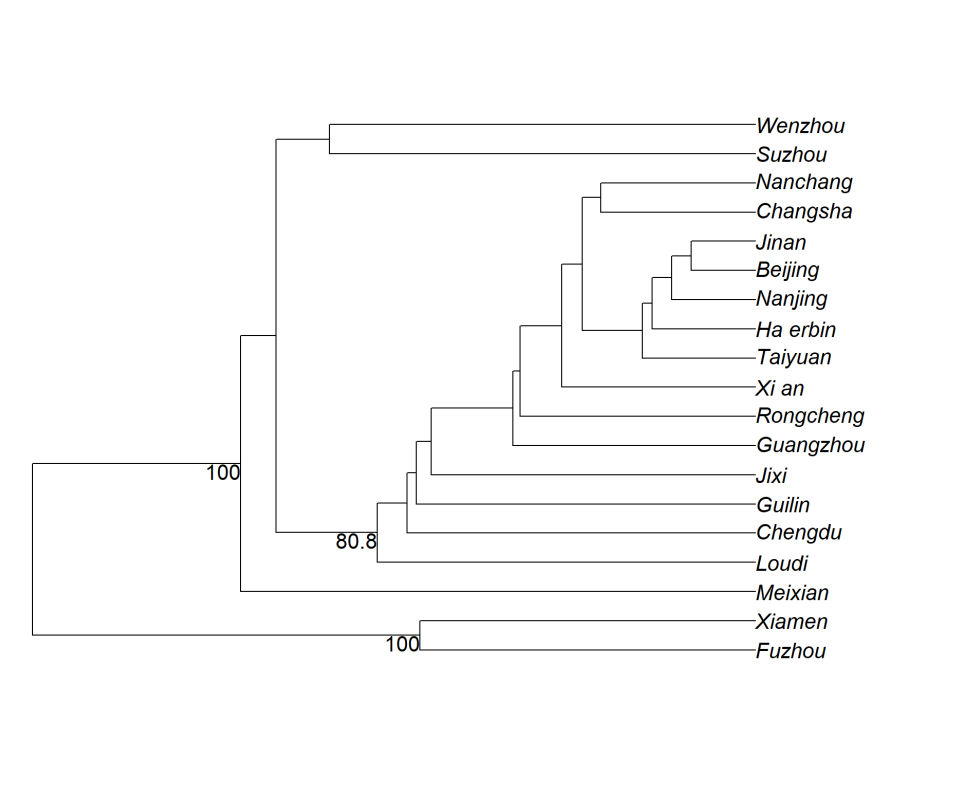
\includegraphics[scale=.2]{Figure/UPGMA_BS_without}
\caption{Sans emprunts}
\end{subfigure}
\caption{Arbres d'UPGMA testés avec la technique de BS}
\label{Fig:UPGMA_BS}
\end{figure}
\end{frame}


\begin{frame}{NJ}
\begin{figure}[htbp]
\flushleft
\begin{subfigure}{.4\textwidth}
\centering
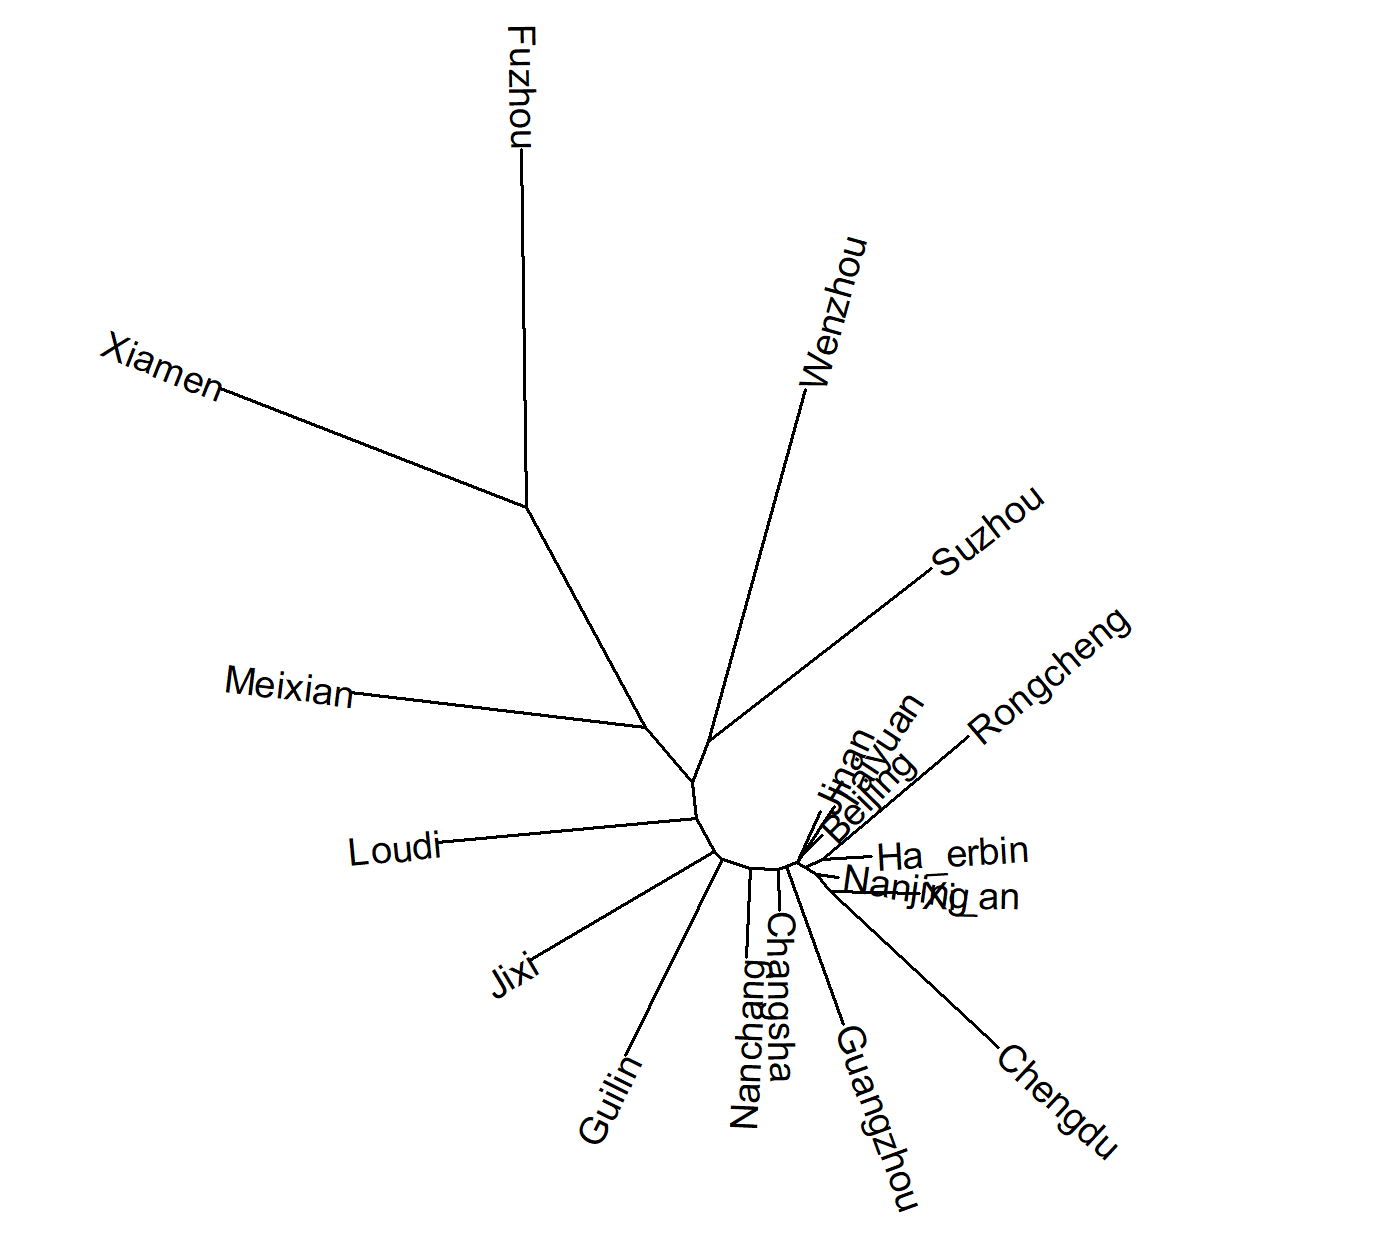
\includegraphics[scale=.12]{Figure/NJ_with}
\caption{Avec emprunts}
\end{subfigure}
\begin{subfigure}{.4\textwidth}
\centering
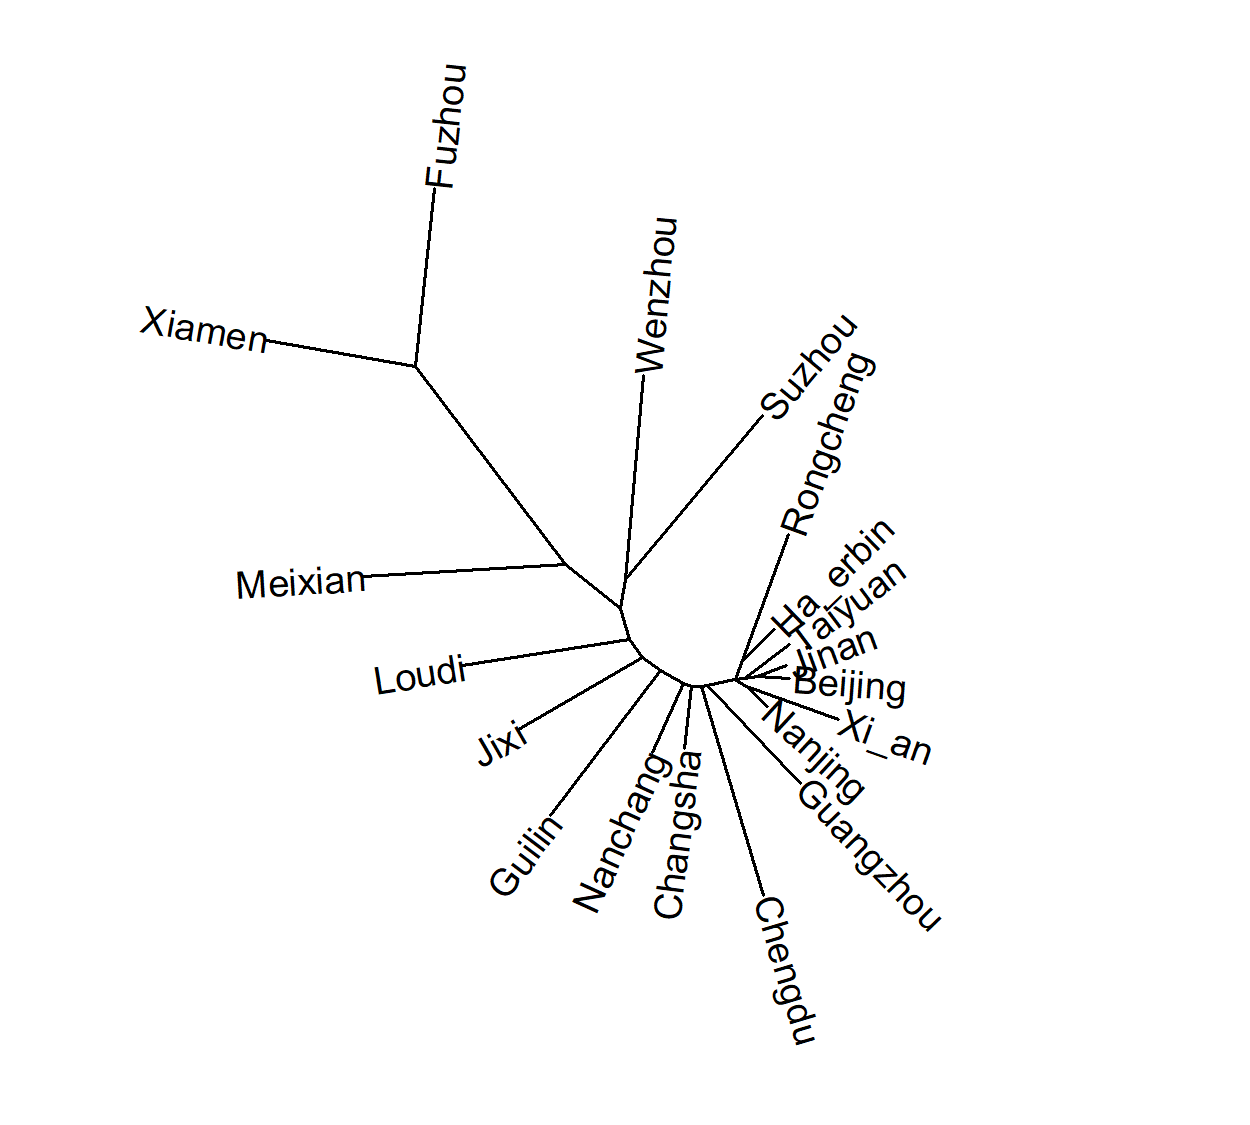
\includegraphics[scale=.15]{Figure/NJ_without}
\caption{Sans emprunts}
\end{subfigure}
\caption{Arbres générés avec la méthode d'NJ}
\label{Fig:NJ}
\end{figure}
\end{frame}

\begin{frame}{MP avec Ratchet}
\flushleft
\begin{figure}
\centering
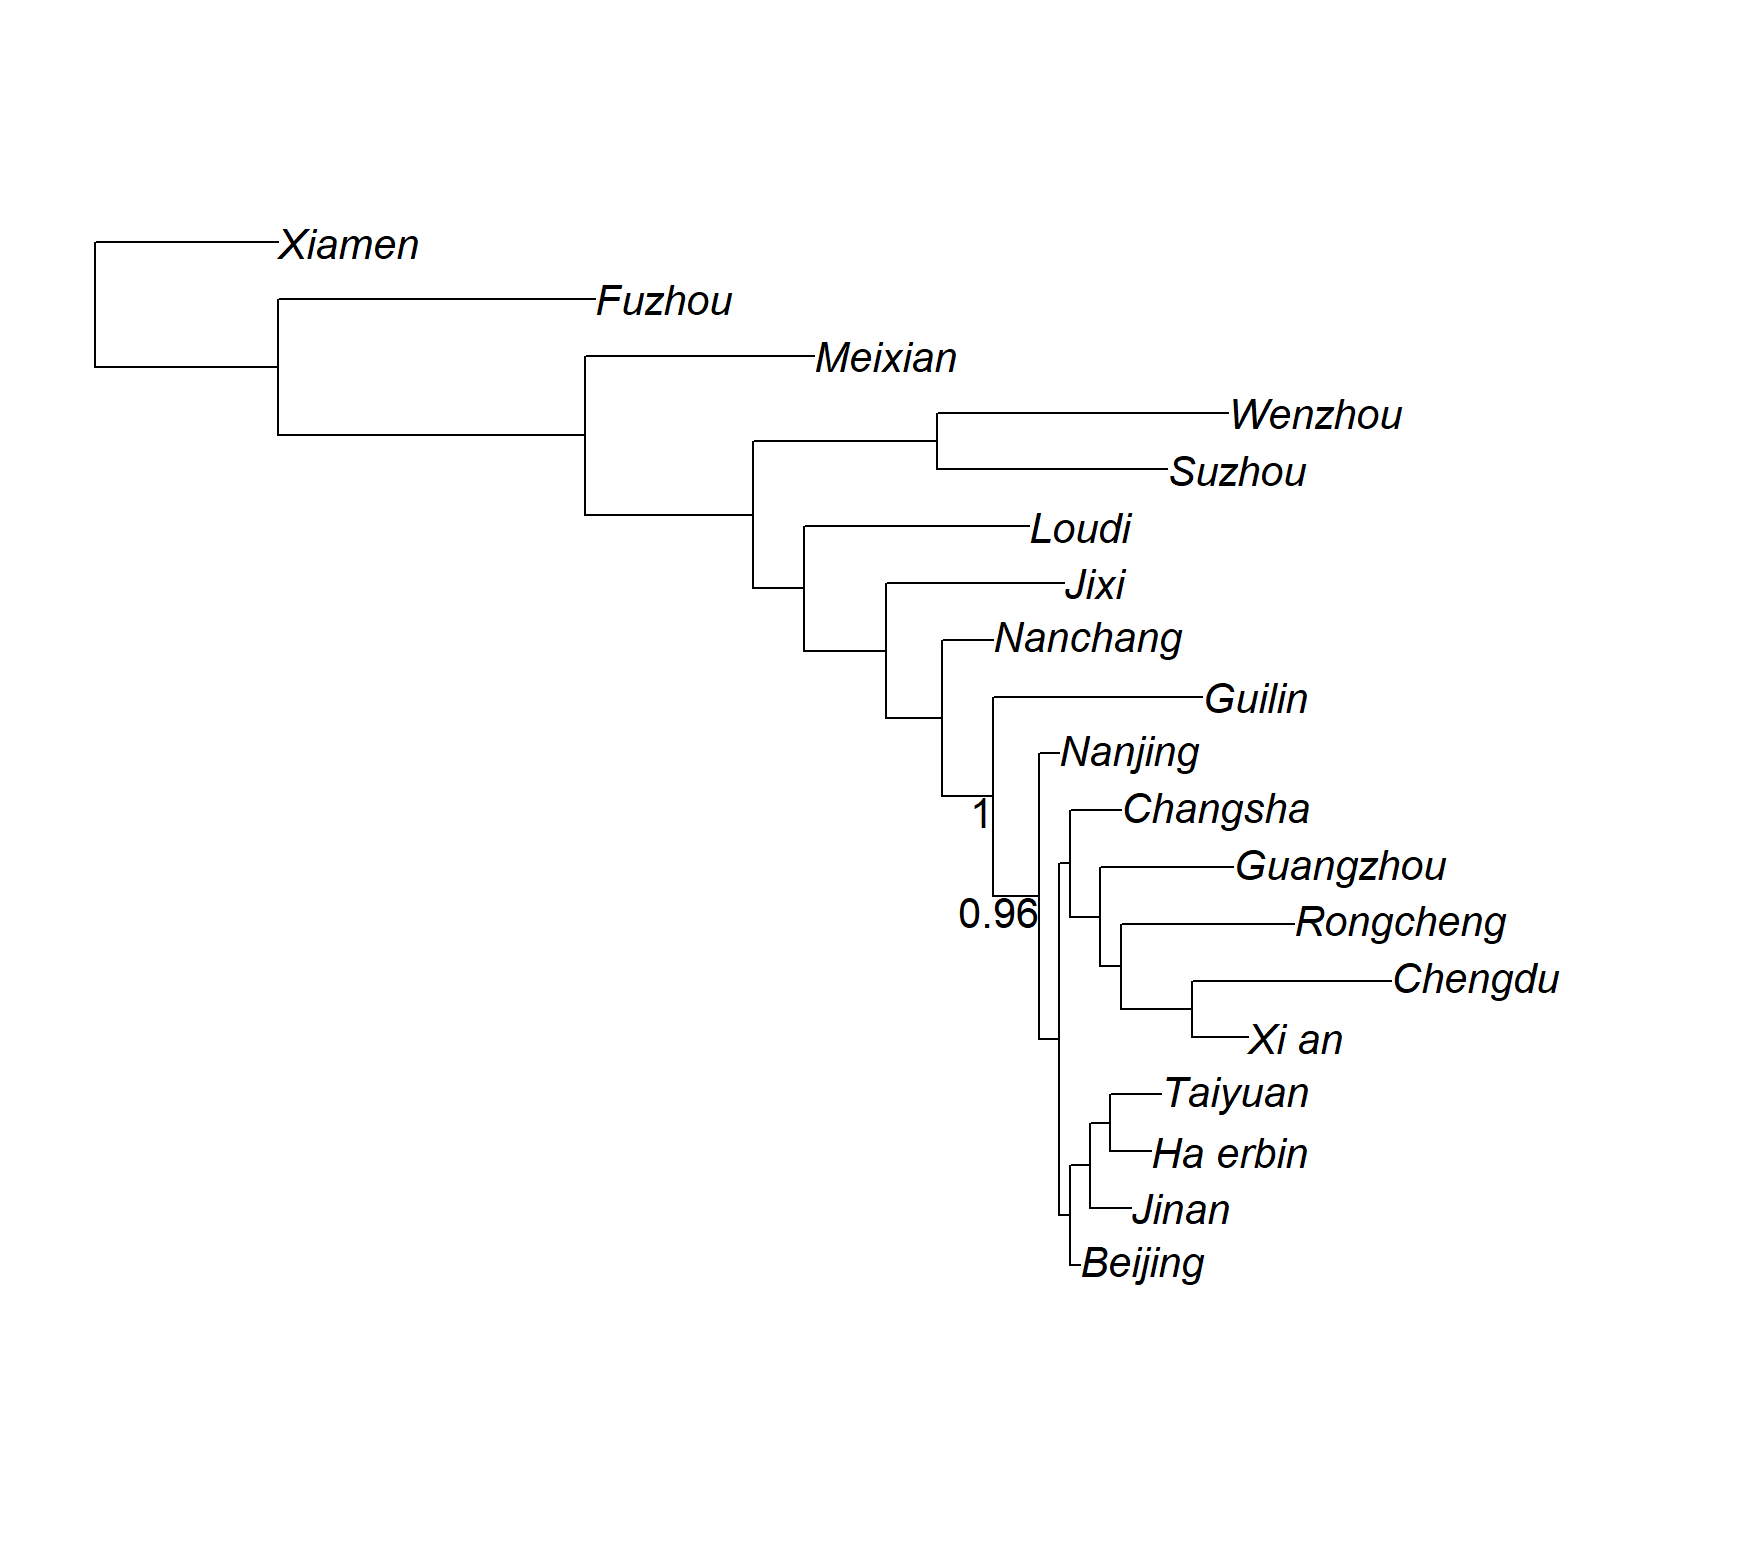
\includegraphics[scale=.15]{Figure/MPR_BS_with}
\caption{Arbres MPR testés avec la technique de BS : avec emprunts}
\label{MPR1}
\end{figure}
\end{frame}

\begin{frame}{MP avec Ratchet}
\begin{figure}
\centering
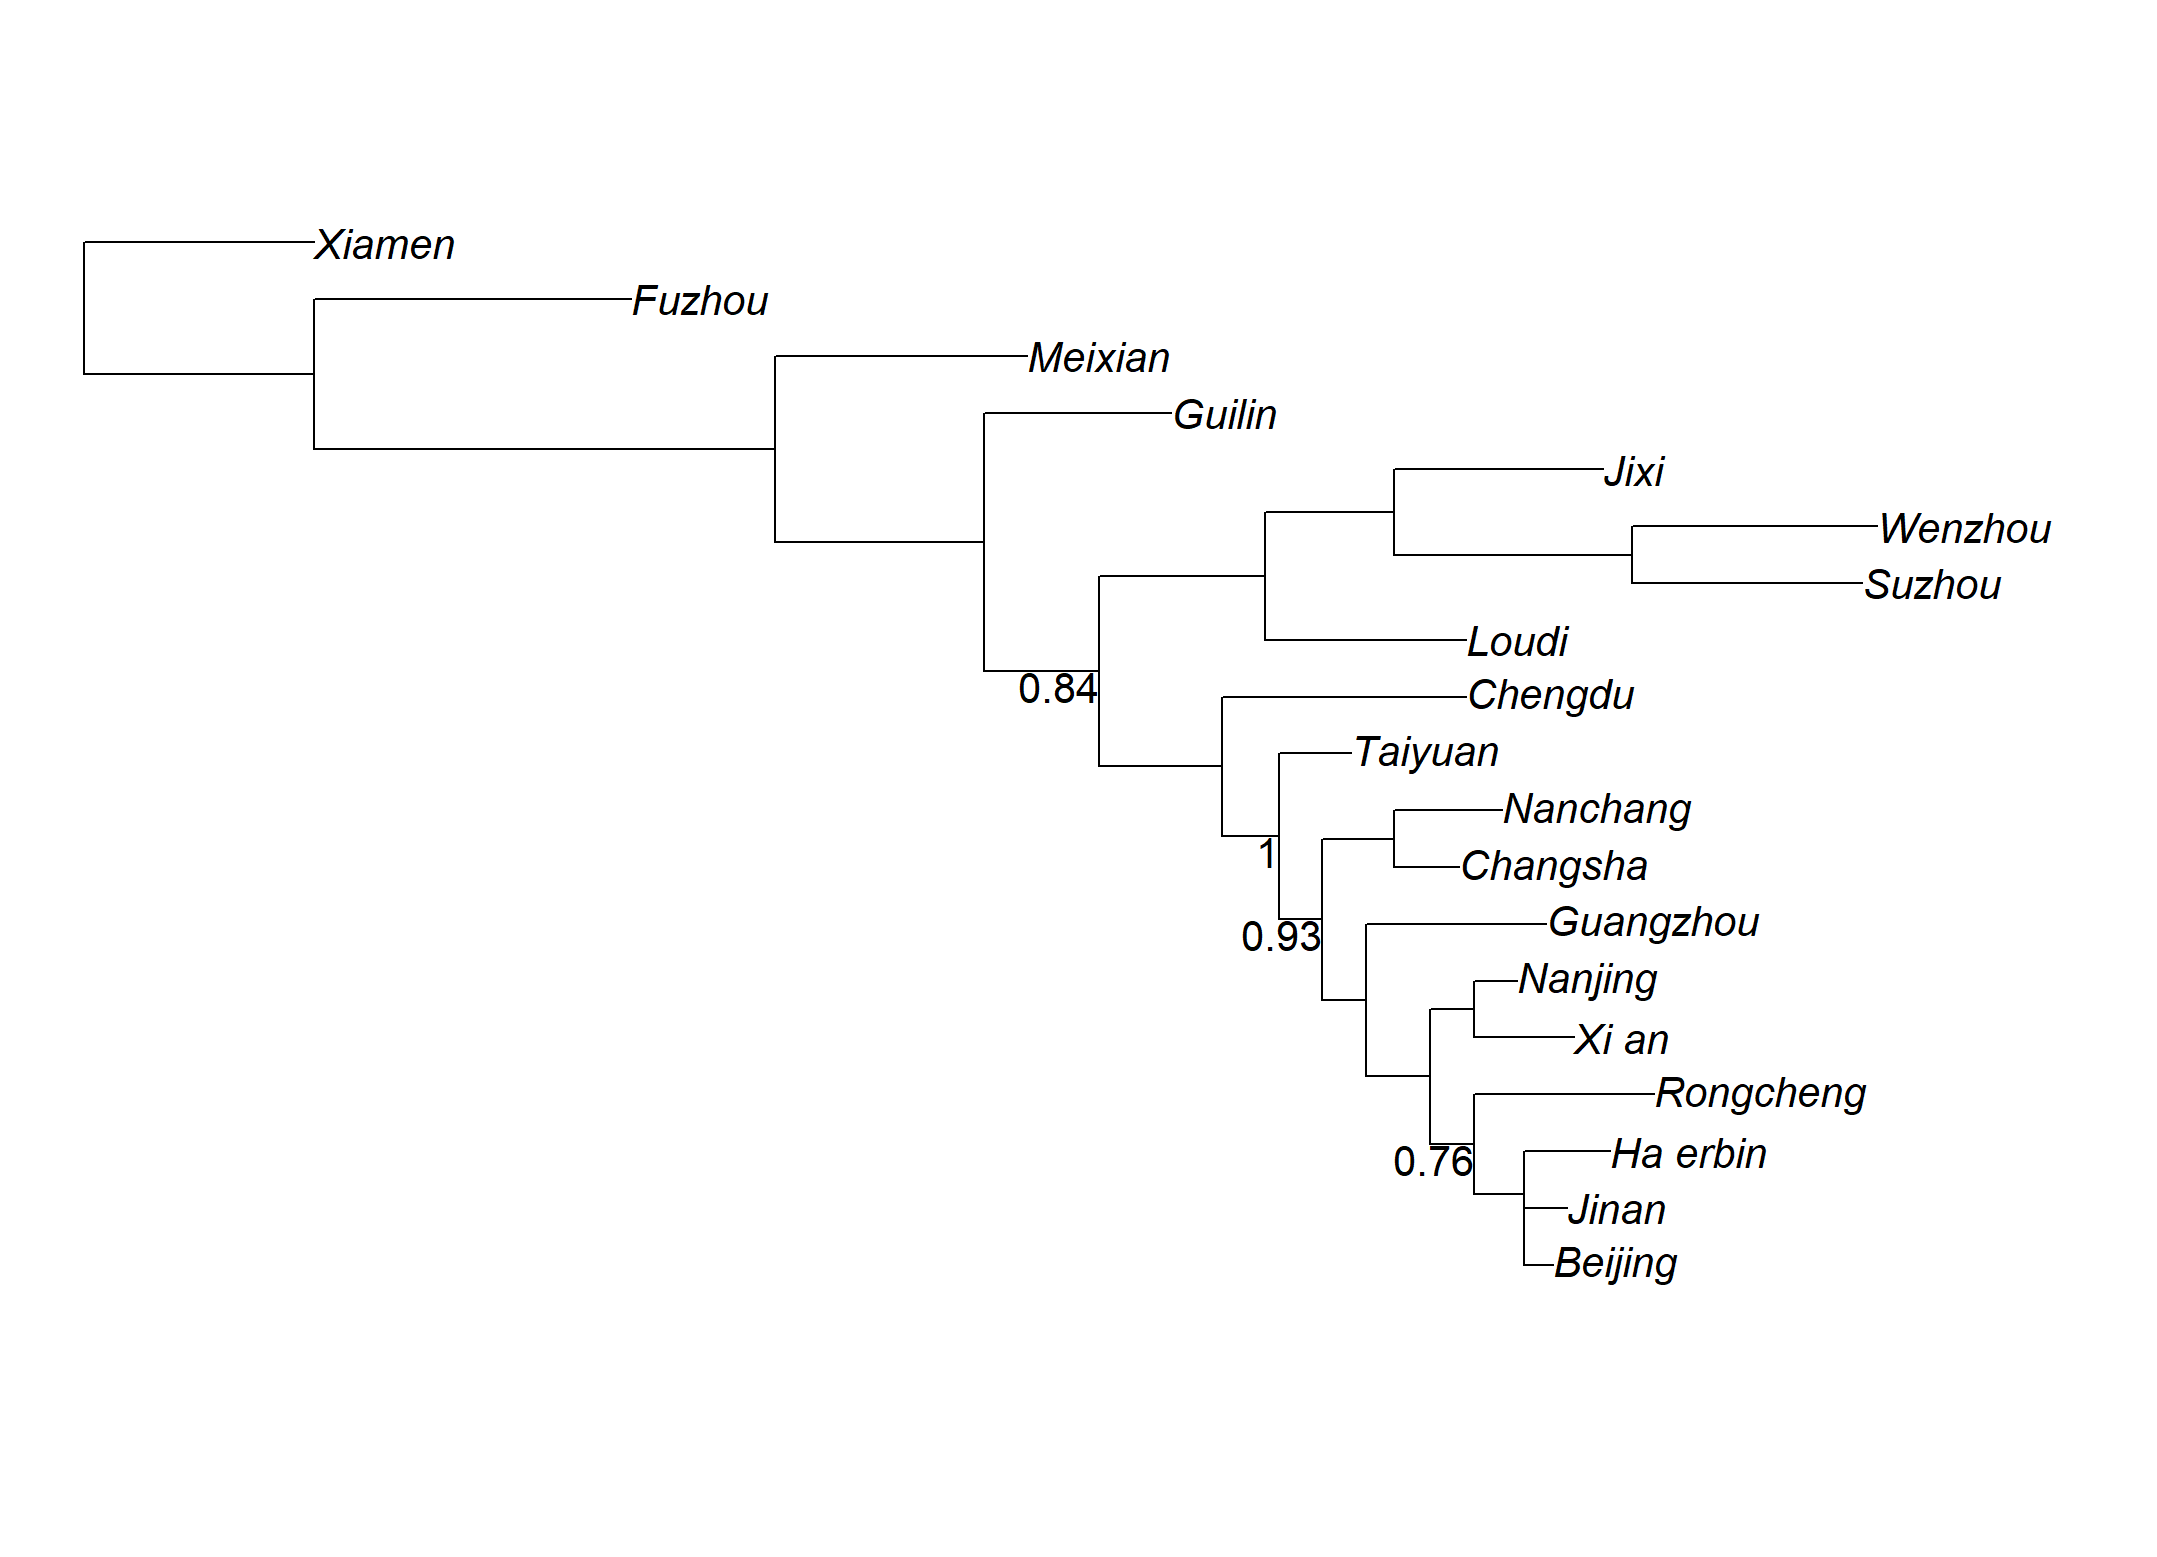
\includegraphics[scale=.15]{Figure/MPR_BS_without}
\caption{Arbres MPR testés avec la technique de BS : sans emprunts}
\label{Fig:MPR2}
\end{figure}
\end{frame}

\begin{frame}{MP avec BaB}
\begin{figure}[htbp]
\flushleft
\begin{subfigure}{.4\textwidth}
\centering
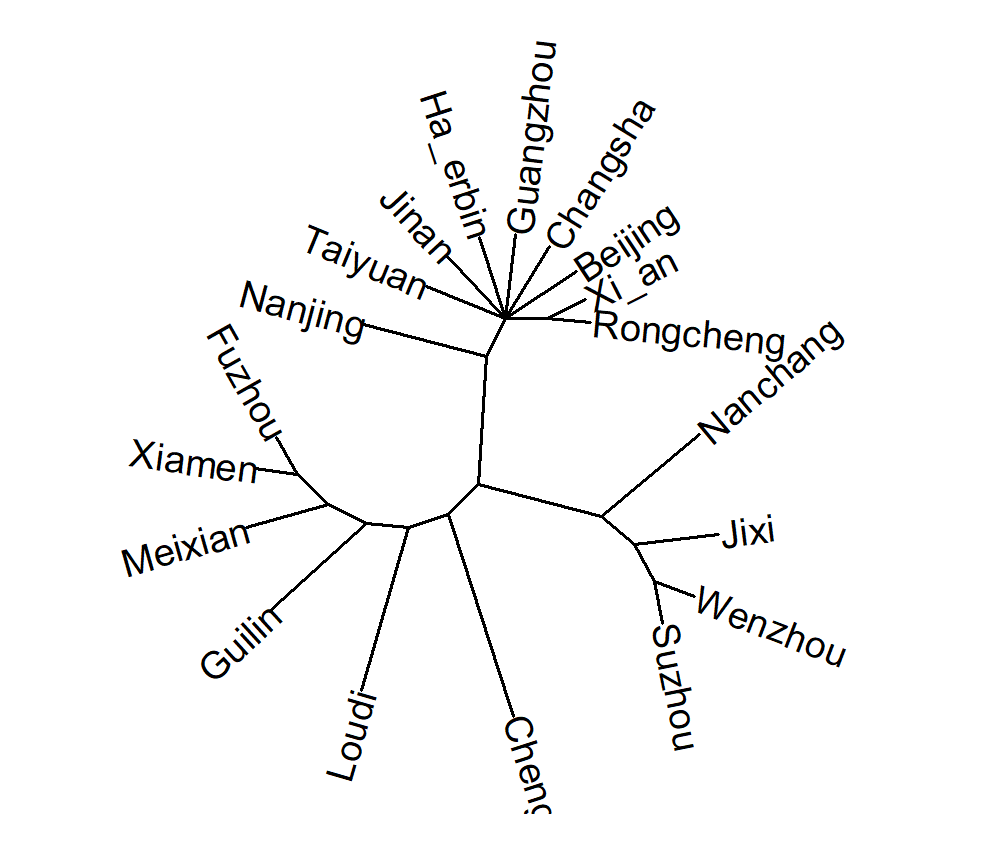
\includegraphics[scale=.2]{Figure/MP_bab_sc_with}
\caption{Avec emprunts}
\end{subfigure}
\begin{subfigure}{.4\textwidth}
\centering
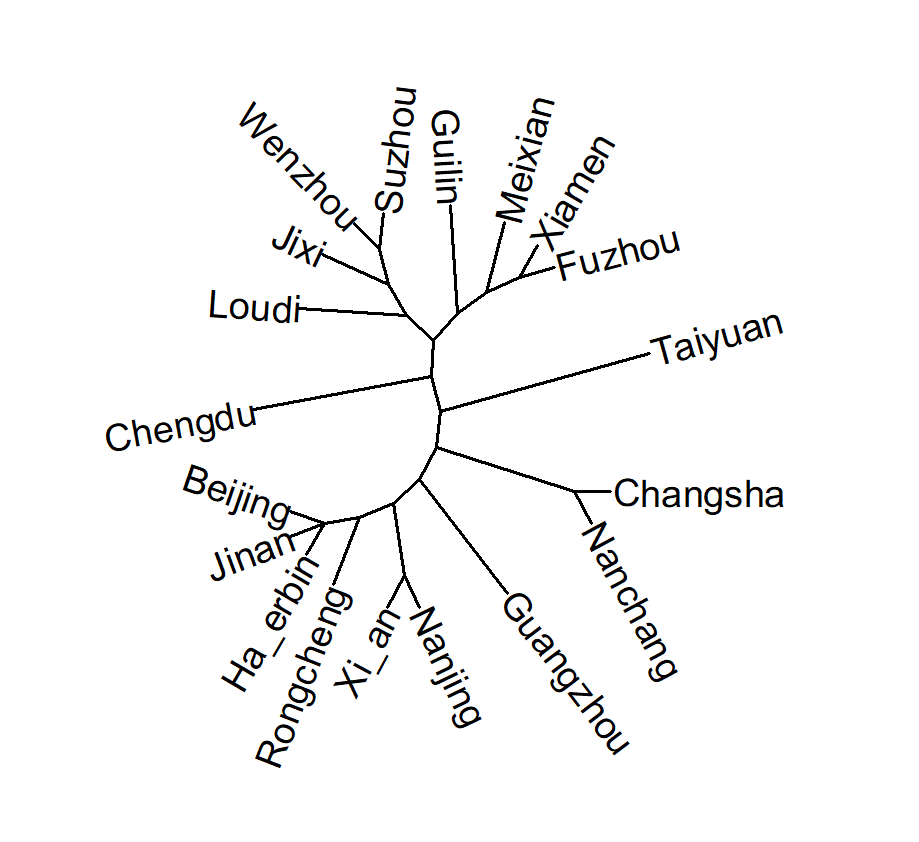
\includegraphics[scale=.2]{Figure/MP_bab_sc_without}
\caption{Sans emprunts}
\end{subfigure}
\caption{Arbres consensus strict des arbres MP}
\label{Fig:MPR_BAB}
\end{figure}
\end{frame}

\begin{frame}{Observation}
\begin{itemize}
\item{Les Min de Fuwhou et Xiamen constituent un clade.}

\item{Les Wu de Suzhou et Wenzhou constituent un clade.}

\item{Le Hakka se sépare après le Min et ne constituent jamais un clade avec le Gan de Nanchang.}

\item{Les Xiang de Changsha et Loudi ne constituent jamais un clade.}
\end{itemize}
\end{frame}

\begin{frame}{Discussion}
\begin{tiny}
Les statuts anormaux du Yue de Guangzhou et du mandarin de Chengdu : 

Deux types de biais résultant de l'écriture dans les enquêtes sur le terrain

    \begin{tabular}{lll}
    \toprule
          & \multicolumn{1}{l}{Avec emprunts} & \multicolumn{1}{l}{Sans emprunts} \\
    \midrule
    Beijing    & 76\%  & 76\% \\
    Jinan      & 74\%  & 75\% \\
    Guangzhou  & \cellcolor[rgb]{ .851,  .851,  .851}70\% & \cellcolor[rgb]{ .851,  .851,  .851}69\% \\
    Rongcheng  & 69\%  & 68\% \\
    \midrule
    Changsha   & 62\%  & 59\% \\
    Nanchang   & 62\%  & 59\% \\
    Jixi       & 61\%  & 61\% \\
    Loudi      & 58\%  & 58\% \\
    Chengdu    & \cellcolor[rgb]{ .851,  .851,  .851}56\% & \cellcolor[rgb]{ .851,  .851,  .851}55\% \\
    Suzhou     & 54\%  & 53\% \\
    \midrule
    Meixian    & 52\%  & 51\% \\
    Wenzhou    & 50\%  & 51\% \\
    Xiamen     & 40\%  & 36\% \\
    Fuzhou     & 22\%  & 32\% \\
    \bottomrule
    \end{tabular}%

e.g. ``给'' v.s. ``畀'' (``donner'') du Yue de Guangzhou
\end{tiny}
\end{frame}

\begin{frame}{Discussion}
\begin{itemize}
\item{La nativisation étymologique des emprunts (\cite{aikio2007etymological})

e.g. ``太阳'' v.s. ``日头/热头'' (``soleil'') du Yue de Guangzhou (\cite[389]{Zhan2002yue}) et du Wu de Suzhou (\cite[346]{Ye1988suzhou_fangyanzhi})
}

\item{Situation opposée : les emprunts détectables partagent la même forme que les mots remplacés

e.g. ``四'' (*sijH) [sɿ] (``quatre'') v.s. ``死'' (*sijX) [si] (``mourir'') du Wu de Suzhou (\cite[96]{Liu2007hexinci})
}
\end{itemize}
\end{frame}

\section{Conclusion}
\begin{frame}{Conclusion}
\begin{itemize}
\item{L'exclusion des emprunts influencerait dans différentes mesures les résultats phylogénétiques.}

\item{Les résultats phylogénétiques confirment dans une mesure ceux de \textcite{sagart2011classifying}.}

\item{Il faut bien veiller à la méthodologie des enquêtes sur le terrain pour obtenir les matériaux pertinents.}

\item{Il faut chercher des solutions aux emprunts indétectables et faussement exclus.}
\end{itemize}
\end{frame}

\section*{Bibliographie}
\begin{frame}[allowframebreaks]{Bibliographie}
\printbibliography
\end{frame}

\end{document}